This test problem is for a homogeneous absorber medium with an incident
flux, which has a simple exponential decay solution.
The problem summary is given in Table \ref{tab:absorber}.

%-------------------------------------------------------------------------------
\begin{table}[htb]\caption{Convergence Test Problem 2 Summary}
\label{tab:absorber}
\centering
\begin{tabular}{l l}\toprule
\emph{Parameter} & \emph{Value}\\\midrule
Domain & $\mathcal{D} = (0,1)$\\
Boundary Conditions & $\scalarsolution(x)=1,\quad x\in\partial\mathcal{D}^-$,\\
   & $\quad\partial\mathcal{D}^-=\{x\in\partial\mathcal{D}:\mathbf{n}(x)
       \cdot\mathbf{\Omega}<0\}$\\
Direction & $\mathbf{\Omega} = \mathbf{e}_x$\\
Cross Section & $\reactioncoef(x)=10$\\
Source & $\scalarsource(x)=0$\\
Speed & $\speed=1$\\
Exact Solution & $\scalarsolution(x)=e^{-10x}$\\
\bottomrule\end{tabular}
\end{table}
%-------------------------------------------------------------------------------

This problem was run in steady-state to avoid temporal error so that spatial
convergence rates could accurately be measured.
The coarsest mesh size in this study uses 8 cells, and each successive mesh
size is halved, with the finest mesh in the study using 256 cells.

Figure \ref{fig:absorber_ss_solution} shows a comparison of the solutions with
32 cells.
The entropy viscosity and Galerkin FCT methods use the analytic solution bounds
given by Equation \eqref{eq:analyticDMP_ss} with the antidiffusion bounds fix given by
Equation \eqref{eq:antidiffusion_bounds_operation}.

%-------------------------------------------------------------------------------
\begin{figure}[ht]
   \centering
      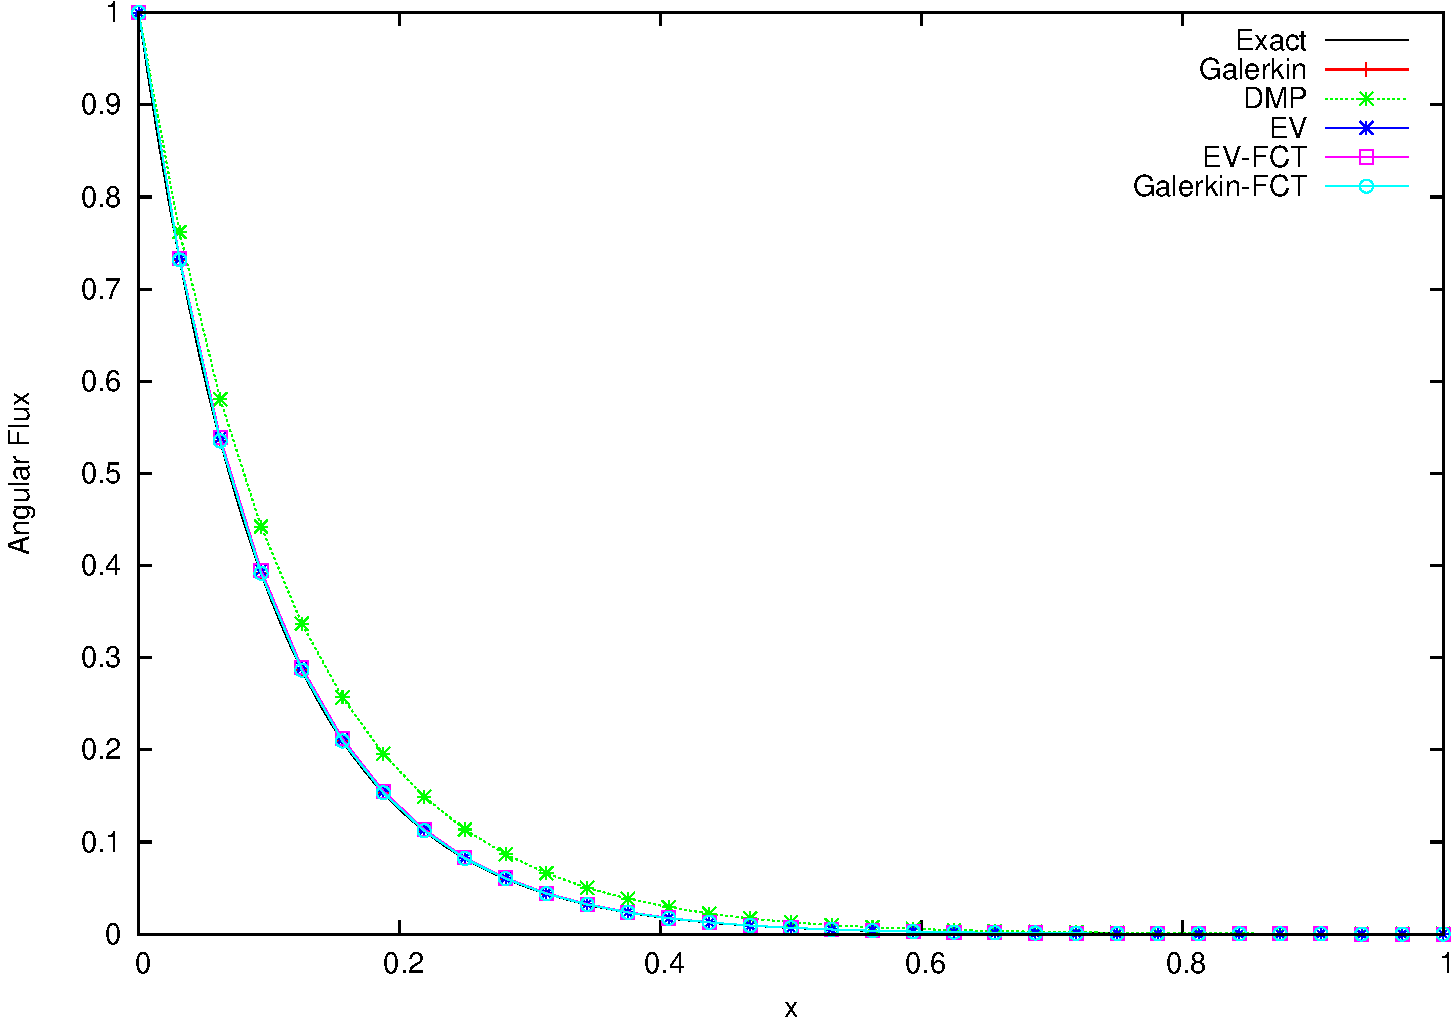
\includegraphics[width=\textwidth]
        {\contentdir/results/transport/absorber_ss/images/angularflux_SS.pdf}
      \caption{Comparison of Solutions for Convergence Test Problem 2 with 32 Cells}
   \label{fig:absorber_ss_solution}
\end{figure}
%-------------------------------------------------------------------------------

Figure \ref{fig:absorber_ss_convergence} shows a comparison of
errors with different methods. The DMP low-order method achieves first-order
spatial convergence as expected, and all other methods achieve second-order
spatial convergence. The entropy viscosity method and the FCT method employing
it both start with more error for the coarsest mesh than the Galerkin method,
but upon refinement, the differences in error diminish.

%-------------------------------------------------------------------------------
\begin{figure}[ht]
   \centering
      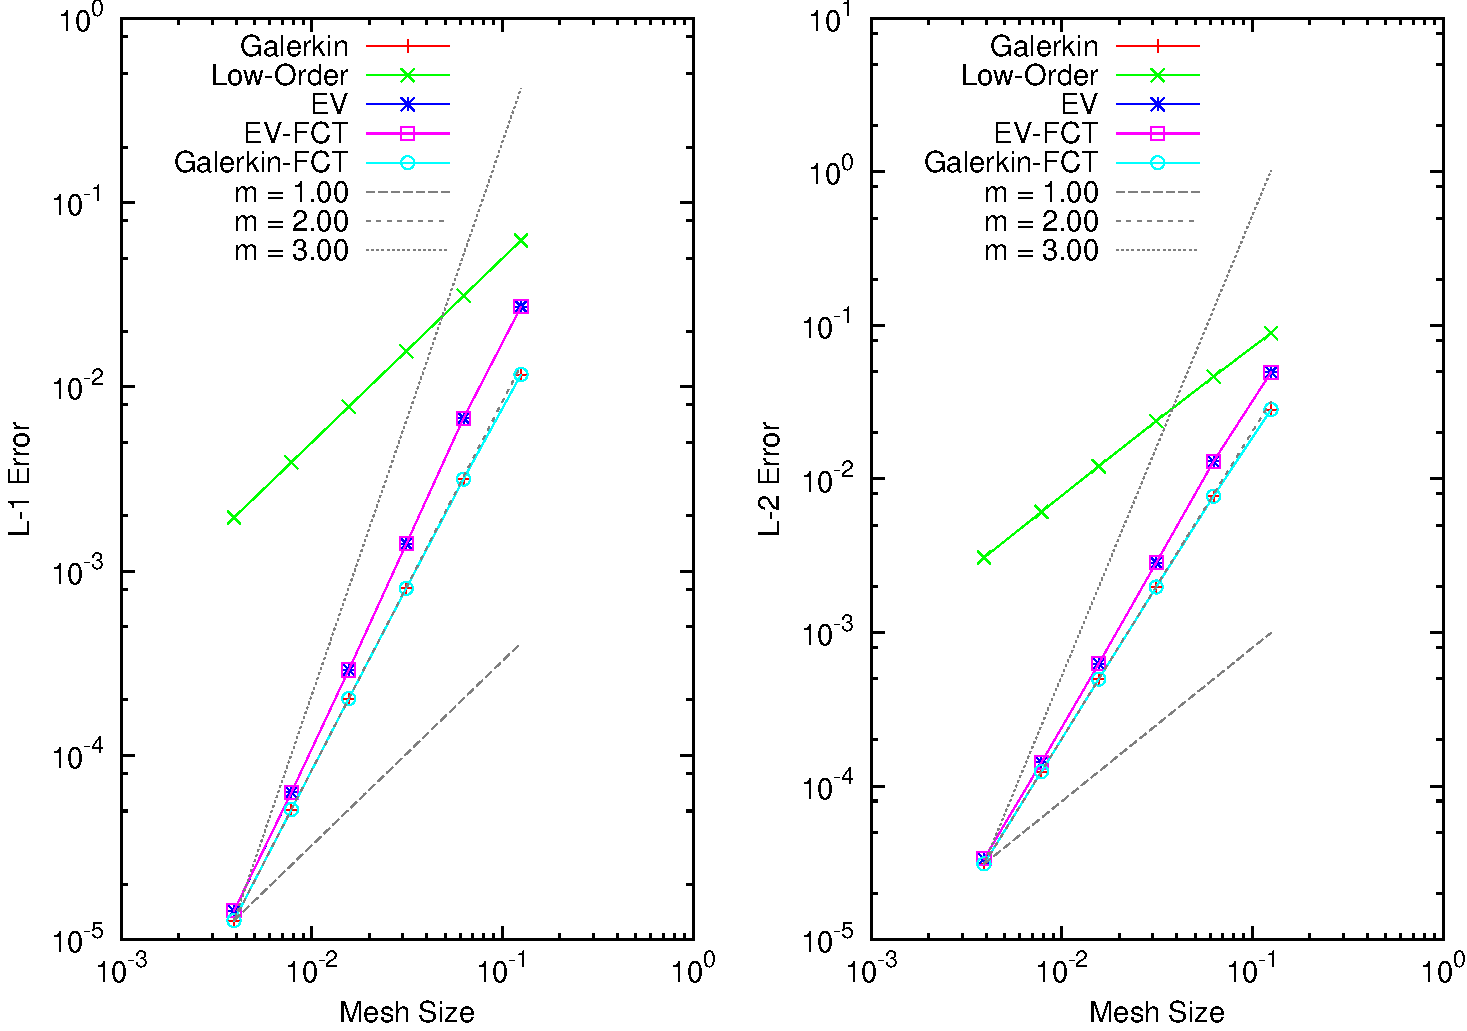
\includegraphics[width=\textwidth]
        {\contentdir/results/transport/absorber_ss/images/convergence_SS.pdf}
      \caption{Comparison of Errors for Convergence Test Problem 2}
   \label{fig:absorber_ss_convergence}
\end{figure}
%-------------------------------------------------------------------------------

\clearpage
